\documentclass{article}
\usepackage[preprint]{neurips_2026}
\usepackage[utf8]{inputenc}
\usepackage[T1]{fontenc}
\usepackage{hyperref}
\usepackage{url}
\usepackage{booktabs}
\usepackage{amsfonts}
\usepackage{amsmath}
\usepackage{amssymb}
\usepackage{nicefrac}
\usepackage{microtype}
\usepackage{graphicx}
\usepackage{xcolor}

\title{Darkness Visible: Reading the Exception Handler of a Language Model}

\author{
  Peter Balogh \\
  \texttt{palexanderbalogh@gmail.com}
}

\begin{document}
\maketitle

\begin{abstract}
The final MLP of GPT-2 Small implements a fully legible routing
program---27 named neurons organized into a three-tier exception handler---while
the knowledge it routes remains entangled across $\sim$3{,}040 residual neurons.
We decompose all 3{,}072 neurons (to numerical precision) into:
5 fused Core neurons that reset vocabulary toward function words,
10 Differentiators that suppress wrong candidates,
5 Specialists that detect structural boundaries, and
7 Consensus neurons that each monitor a distinct linguistic dimension.
The consensus-exception crossover---where MLP intervention shifts from helpful
to harmful---is statistically sharp (bootstrap 95\% CIs exclude zero at
all consensus levels; crossover between 4/7 and 5/7).
Three experiments show that ``knowledge neurons'' \citep{dai2022knowledge} are
routing infrastructure, not fact storage: the MLP amplifies or suppresses
signals already present in the residual stream from attention, with capability
indexed by contextual constraint (succeeding when only one completion is
plausible, failing on arbitrary associations).
A garden-path experiment reveals a \emph{reversed} garden-path effect---GPT-2
uses verb subcategorization immediately, consistent with the exception handler operating at token-level predictability
rather than syntactic structure.
The developmental arc across layers is confirmed under the tuned lens of
\citet{belrose2023eliciting}.
This architecture crystallizes only at the terminal layer---in deeper models,
we predict equivalent structure at the final layer, not at layer~11.
Code and data: \url{https://github.com/pbalogh/transparent-gpt2}.
\end{abstract}

%=============================================================================
\section{Introduction}
%=============================================================================

The MLP layers of transformer language models are typically treated as opaque
nonlinear transformations.
Recent work has shown that individual neurons can be interpreted
\citep{gurnee2023finding, bricken2023monosemanticity}, that MLP layers implement
key-value memories \citep{geva2021transformer}, and that specific factual
associations can be located and edited \citep{meng2022locating}.
But a complete, legible account of an MLP layer's \emph{routing logic}---readable
as pseudocode with named variables---has remained elusive.

We provide such an account for Layer~11 of GPT-2 Small, the model's final MLP, while showing that the knowledge it routes remains distributed across $\sim$3{,}040 residual neurons.
Our decomposition preserves the original weights to numerical precision while revealing
a routing architecture that overturns several assumptions:

\begin{enumerate}
\item \textbf{MLP layers are not opaque.}
A single exception neuron reliably signals which processing path is active,
seven consensus neurons each monitor a distinct linguistic dimension, and
20 exception-handler neurons organize into three functional tiers
(Figure~\ref{fig:pseudocode}).
This routing program is diagnostic, not causal \citep{balogh2026discrete}.
The pseudocode in Figure~\ref{fig:pseudocode} captures the functional
organization --- how neurons coordinate into a routing program --- even though
no single neuron is a causal bottleneck.

\item \textbf{``Knowledge neurons'' are routing infrastructure.}
Neurons identified by \citet{dai2022knowledge} as storing factual knowledge
appear across nearly all facts tested---they are highway signs, not warehouses.
This reframes ROME \citep{meng2022locating}: editing MLP weights changes
routing decisions, not stored facts.

\item \textbf{The exception handler has sharp scope boundaries.}
It detects token-level predictability (subword fragments, structural breaks)
but not syntactic reparse: garden-path sentences produce a \emph{reversed}
effect, suggesting GPT-2 Small behaves as a one-stage parser for verb
subcategorization ambiguities (\S\ref{sec:garden_path}).

\item \textbf{Routing legibility is unique to the terminal layer.}
A survey across all 12 layers shows no comparable structure at any earlier
layer---a phenomenon we call \emph{terminal crystallization}, with a testable
depth-tracking prediction.
\end{enumerate}

\begin{figure}[t]
\centering
\small
\begin{verbatim}
 ROUTING PROGRAM: L11 MLP (27 named neurons)
 -------------------------------------------
 consensus = count(N2, N2361, N2460, N2928,
                   N1831, N1245, N2600)
 exception = N2123.fires    // 11.3% of tokens

 if exception:
   // N2123 is a diagnostic readout, not a causal gate
   CORE(N2123,N2910,N740,N1611,N2044):
     reset vocab -> {the, in, and, a, ,}
     // 54% of output norm, +0.2% PPL
   DIFF(N2462, N2173, N1602, N1800, N2379,
        N1715, N611, N3066, N584, N2378):
     suppress wrong candidates
     repair subword fragments
     // 23% of output norm, +1.3% PPL
   SPEC(N2921,N2709,N971,N2679,N737):
     detect paragraph/clause boundaries
     // 4% of output norm, -0.3% PPL
 else:
   // consensus >= 5/7: MLP intervention
   // is counterproductive (dP < 0)
   // but architecture has no bypass

 RESIDUAL(~3,040 neurons):
   amplify/suppress attention-derived signal
   // distributed, not individually legible
\end{verbatim}
\caption{The exception handler as pseudocode. Consensus neurons vote
on linguistic predictability; the exception neuron signals the processing
path. The 20 exception-handler neurons are individually characterizable;
the $\sim$3,040 residual neurons are not. Braces denote the vocabulary
distribution each tier pushes toward. PPL impact from Table~\ref{tab:ablation}.
The pseudocode represents the \emph{functional organization} observed in
activation patterns, not a literal causal program: N2123 reliably indicates
which path is active but does not control it.}
\label{fig:pseudocode}
\end{figure}

\begin{quote}
\emph{``No light, but rather darkness visible.''}
\hfill ---Milton, \emph{Paradise Lost}
\end{quote}

\noindent Language models are routinely called ``black boxes''---as if the darkness
inside were uniform.
It is not.
Inside L11's MLP we find \emph{structured} darkness: a legible routing
program wrapped around knowledge that is distributed across $\sim$3{,}000
residual neurons and cannot be decomposed into named units.
The darkness is visible precisely because it has structure.
We can delineate what navigates the dark, even when the dark itself
remains opaque.

%=============================================================================
\section{Background}
%=============================================================================

\paragraph{MLP interpretability.}
\citet{geva2021transformer} showed that MLP layers act as key-value memories,
with the first projection (W$_\text{fc}$) computing keys and the second
(W$_\text{proj}$) storing values.
\citet{geva2023dissecting} refined this picture, tracing factual recall
step by step through attention and MLP layers and finding that MLPs at
subject-last positions promote correct attributes---a more nuanced view
than our binary ``routing vs.\ retrieval'' framing.
\citet{meng2022locating} demonstrated that factual associations can be edited
via rank-one MLP weight updates (ROME), raising the question of whether editing
changes stored knowledge or routing behavior---a tension we address in \S\ref{sec:knowledge}.
\citet{dai2022knowledge} identified ``knowledge neurons'' in BERT MLPs using
integrated gradients, claiming individual neurons are necessary for specific
facts. Our \S\ref{sec:knowledge_neurons} tests this on GPT-2 and finds that
the same neurons appear across diverse facts---they are routing infrastructure,
not fact-specific storage.
\citet{bricken2023monosemanticity} decomposed MLP activations using sparse
autoencoders, revealing monosemantic features in superposition.
\citet{templeton2024scaling} extended this approach to production-scale models,
finding interpretable features across Claude 3 Sonnet---suggesting that SAE
decomposition could potentially resolve further structure within
the $\sim$3{,}040 residual neurons that our manual analysis cannot decompose.
\citet{bills2023language} showed that GPT-4 can generate natural-language
descriptions of individual neurons, complementing the enrichment-based
characterization we use here.

\paragraph{Transformer circuits.}
\citet{elhage2021mathematical} introduced the residual stream framework and
the mathematical tools (OV/QK factorization) for mechanistic analysis of
transformers. \citet{olsson2022context} extended this to identify induction
heads as a fundamental circuit motif.
\citet{wang2023interpretability} provided a complete circuit-level account
of indirect object identification in GPT-2 Small---the same model we study---tracing
the behavior through 26 attention heads. Where they traced a \emph{circuit}
(a behavior across layers), we trace an \emph{entire layer} (all behaviors
within L11's MLP).
\citet{conmy2023automated} introduced automated methods (ACDC) for circuit
discovery; we deliberately use manual characterization to demonstrate full
legibility, though automated methods could scale the approach.
Other circuit-level analyses of GPT-2 include \citet{hanna2024does} on
greater-than comparison and \citet{merullo2024circuit} on component reuse
across tasks.
\citet{nanda2023progress} demonstrated that interpretability can track
learning dynamics, a connection to our developmental arc analysis.

\paragraph{Binary routing.}
\citet{balogh2026discrete} identified a consensus/exception architecture in
GPT-2 Small's L11 MLP: 7 consensus neurons whose agreement predicts a 94.3
percentage-point drop in exception neuron firing (95\% CI: [93.8, 94.7]),
with the MLP becoming counterproductive at full consensus.
\citet{dettmers2022llm} found that a small number of outlier features account for
most activation magnitude, a pattern compatible with sparse binary routing.
The present paper extends \citet{balogh2026discrete} from \emph{detecting} the
routing structure to \emph{reading} it---characterizing every neuron in the
exception handler and documenting what each one does.
Critically, \citet{balogh2026discrete} showed that N2123 is diagnostic rather
than causal: zeroing it alone has no measurable effect on perplexity ($<$0.1\%).
The routing structure is real but emerges from the distributed activity of all
3,072 neurons; N2123 is a reliable readout of this collective computation,
not a bottleneck that controls it.

\paragraph{Layer-wise development.}
\citet{tenney2019bert} showed that BERT rediscovers the classical NLP pipeline
across layers: POS tagging in early layers, parsing in middle layers, and
semantic tasks later. Our three-phase developmental arc (scaffold $\to$
decision $\to$ terminal crystallization) extends this finding to GPT-2's
MLP layers, with the additional observation that routing legibility is
concentrated at the terminal layer.

\paragraph{Attention sinks and head specialization.}
\citet{xiao2023efficient} identified the attention sink phenomenon: certain
positions (typically BOS) absorb disproportionate attention mass, serving as
no-op destinations.
\citet{clark2019what} and \citet{voita2019analyzing} showed that attention
heads specialize for different functions, with many heads prunable.
L11's most important attention head (L11H7, 6$\times$ the importance
of any other head) sends 45\% of its weight to BOS---an instance of the
sink phenomenon.

%=============================================================================
\section{Methods}
%=============================================================================

\subsection{Transparent Forward Pass}

We construct a \textsc{TransparentGPT2} that wraps GPT-2 Small (124M parameters)
with no weight modifications.
At Layer~11, the MLP's output is decomposed into tier contributions:
\begin{equation}
\text{MLP}(x) = \underbrace{\text{Core}(x)}_{\text{5 neurons}} +
\underbrace{\text{Diff}(x)}_{\text{10 neurons}} +
\underbrace{\text{Spec}(x)}_{\text{5 neurons}} +
\underbrace{\text{Residual}(x)}_{\text{3,052 neurons}}
\end{equation}
Each tier applies a binary mask to the post-GELU activations before projecting
through the output matrix.
The sum equals the original MLP output exactly
(maximum elementwise difference $< 6 \times 10^{-5}$,
cosine similarity 0.99999994).

\subsection{Data and Neuron Characterization}

All experiments use 512,000 tokens from WikiText-103, processed in 500 sequences
of 1,024 tokens each (respecting GPT-2's positional embedding limit).
Forward hooks capture pre-GELU activations at the target layer.
Binary firing is determined by $|\text{GELU}(x_n)| > 0.1$;
we verify robustness of all structural findings across thresholds
$\theta \in \{0.01, 0.05, 0.1, 0.25, 0.5, 1.0\}$ in \S\ref{sec:threshold}.

\paragraph{Two activation regimes for N2123.}
A distinction matters for interpreting enrichment statistics.
At the generic threshold ($|\text{GELU}| > 0.1$), N2123 activates on 70.9\% of tokens---it is broadly responsive.
However, only 11.3\% of tokens produce the \emph{high-magnitude} activations
(top decile of N2123's activation distribution)
that reliably co-occur with exception-path behavior:
Core co-firing, Differentiator engagement, and consensus suppression.
Throughout \S\ref{sec:exception}--\S\ref{sec:knowledge}, ``exception path active''
refers to this high-magnitude regime (11.3\%).
The enrichment analysis in Table~\ref{tab:enrichment_stats} uses the generic
$> 0.1$ threshold for consistency with the other 3{,}071 neurons;
the resulting 1.41$\times$ enrichment for N2123 reflects the modest increase
from 70.9\% to 100\% under this definition, and should not be confused with
the routing-relevant high-magnitude firing.
Co-firing structure is measured by Jaccard similarity between neuron firing
patterns across all tokens.

\paragraph{Enrichment analysis.}
For each neuron $n$ and condition $C$ (e.g., ``exception neuron fires''),
enrichment is the frequency ratio
$E(n, C) = P(n \text{ fires} \mid C) \,/\, P(n \text{ fires})$.
Statistical significance is assessed by one-sided Fisher's exact test on the
$2 \times 2$ contingency table (fires/silent $\times$ condition/baseline),
with Bonferroni correction for 3{,}072 neurons ($\alpha = 0.05 / 3072 \approx
1.6 \times 10^{-5}$).

\paragraph{Bootstrap inference.}
All confidence intervals use sequence-level bootstrap (10{,}000 resamples,
resampling 500 sequences with replacement) to account for within-sequence
autocorrelation. Individual tokens within a sequence share context and are
not independent; resampling at the sequence level produces conservative CIs.
Six of 27 routing neurons are significantly enriched under exception firing
at this threshold (Table~\ref{tab:enrichment_stats}); notably, consensus neurons
are \emph{not} enriched, as predicted by the consensus-exception anticorrelation
reported in \citet{balogh2026discrete}.

\subsection{Cross-Layer Replication}

To test whether the exception handler architecture is unique to L11, we replicate
the full characterization analysis at L7 and L10---the other layers identified by
\citet{balogh2026discrete} as having consensus structure.

\subsection{Consensus Neuron Profiling}

For each of the 7 consensus neurons, we compute:
(a) enriched tokens---those overrepresented when the neuron fires versus its base rate;
(b) depleted tokens---those underrepresented;
(c) output direction---the vocabulary distribution the neuron pushes toward,
computed by projecting its column of W$_\text{proj}$ through layer norm and the
unembedding matrix.

\subsection{Knowledge Extraction Test}

For 160 diverse factual cloze prompts spanning 15 categories, we progressively
accumulate residual neuron contributions and track whether the correct token's
rank improves.
We conduct both a \emph{static} version (accumulating raw $W_\text{proj}$ columns)
and a \emph{context-dependent} version (scaling each column by the neuron's actual
post-GELU activation for the given prompt).
This tests the hypothesis that factual knowledge is stored combinatorially in
residual neurons.

%=============================================================================
\section{The Exception Handler}
\label{sec:exception}
%=============================================================================

\subsection{Three-Tier Architecture}

Among the 11.3\% of tokens where the exception neuron N2123 fires, the remaining
neurons organize into three tiers by conditional fire rate (Table~\ref{tab:tiers}).

\begin{table}[t]
\centering
\caption{Three-tier exception handler at L11. Fire rates are conditional on
N2123 firing. Jaccard similarity is with N2123.}
\label{tab:tiers}
\small
\begin{tabular}{@{}llcccl@{}}
\toprule
Tier & Neurons & Count & Fire Rate & Jaccard & Function \\
\midrule
Core & N2123, N2910, N740, & 5 & 90--100\% & $\geq$0.91 & Vocabulary reset \\
     & N1611, N2044 & & & & \\
Differentiator & N2462, N2173, N1602, N1800, & 10 & 35--88\% & 0.15--0.89 & Candidate suppression, \\
     & N2379, N1715, N611, N3066, & & & & subword repair, \\
     & N584, N2378 & & & & suppression \\
Specialist & N2921, N2709, N971, & 5 & 14--37\% & $<$0.15 & Boundary detection \\
     & N2679, N737 & & & & \\
\bottomrule
\end{tabular}
\end{table}

\paragraph{Core: a fused mega-neuron.}
The 5 Core neurons fire on 90--100\% of exception tokens and exhibit pairwise
Jaccard similarities $\geq 0.91$ (peak: N2123$\leftrightarrow$N2910 at 0.998).
They are functionally a single unit.
Their output directions all push toward generic function words:
\texttt{the}, \texttt{in}, \texttt{and}, \texttt{a}, \texttt{,}.
This is a \textbf{vocabulary reset}---shifting the prediction distribution toward
a generic prior before the residual contributes contextual adjustments.
The Core accounts for 54\% of the exception-path output norm, though its PPL
impact is modest (+0.2\%, \S\ref{sec:ablation})---most of its large-magnitude
signal is a DC offset toward function words that the residual stream already
provides.
The Core establishes the baseline vocabulary distribution; the Differentiators
(\S\ref{sec:ablation}) do the discriminative work.

\paragraph{Differentiators: suppression, not promotion.}
The 10 Differentiator neurons include a suppression pair
(N584$+$N2378, Jaccard 0.889) and subword repair neurons (N1602, N1715).
They contribute 23\% of exception-path output norm.
Their role is to suppress wrong candidates rather than promote correct ones,
narrowing the vocabulary space that the residual neurons then fill.

\paragraph{Specialists: boundary detection.}
N737 is a solo paragraph boundary detector (Jaccard $< 0.15$ with all other
neurons), firing independently at structural transitions.
The Specialists contribute only 4\% of output norm but handle structurally
critical positions.

\subsection{The Exception Indicator}

N2123's output direction pushes toward function words
(\texttt{,} at +3.0, \texttt{the} at +2.7, \texttt{and} at +2.7)
and suppresses byte-pair artifacts and garbage tokens (logits $\sim -6$).
Its input sensitivity (from W$_\text{fc}$) responds to subword fragments
(\texttt{anny}, \texttt{arter}, \texttt{idd}) and is inhibited by complete
content words (\texttt{destro[y]}, \texttt{challeng[e]}, \texttt{conclud[e]}).

\textbf{Interpretation:} N2123 detects tokens where the model ``doesn't yet know
what's happening''---incomplete words, structural breaks, rare patterns.
Its firing pattern reliably indicates which processing path is active, but
it is not a causal bottleneck: zeroing N2123 alone changes perplexity by
$<$0.1\%, and clamping it ON for consensus tokens has no measurable effect
\citep{balogh2026discrete}.
N2123 is best understood as a \textbf{vote counter}---a readable summary of
the distributed routing decision made collectively by all 3,072 neurons.
Removing the counter does not change the election.

\subsection{Progressive Prediction}

We demonstrate the tier-by-tier construction of predictions on factual prompts.
For ``In 1969, astronauts landed on the \underline{\hspace{1cm}}'':

\begin{itemize}
\item \textbf{Before MLP}: Residual stream predicts \texttt{moon} (from attention)
\item \textbf{After Core}: Prediction shifts toward \texttt{the} (vocabulary reset)
\item \textbf{After Differentiators}: Wrong candidates suppressed
\item \textbf{After Residual}: Prediction returns to \texttt{moon}, now with
redistributed probability mass
\end{itemize}

The Core acts as a \textbf{DC offset}: it shifts the entire distribution toward
a safe function-word prior that the residual stream then overrides with
context-specific content.
Its large output norm (54\%) but minimal PPL impact (+0.2\%) reflects this
role---it is a floor, not a ceiling, and the residual stream's contextual
signal overwrites it.
Across 12 factual prompts tested systematically, 10/12 show this
Core$\to$reset$\to$Differentiator$\to$suppress pattern; the 2 exceptions
involve subword-initial predictions where the Core's function-word push
has no effect (the target is a BPE fragment, not a function word).
Named circuits handle routing and vocabulary management; factual knowledge
lives in the $\sim$3{,}040 residual neurons.

%=============================================================================
\section{The Consensus Detector}
\label{sec:consensus}
%=============================================================================

\subsection{Seven Dimensions of Normal}

Each consensus neuron monitors a distinct linguistic property
(Table~\ref{tab:consensus}), characterized via enrichment/depletion analysis
and disagreement patterns across 512,000 tokens.
The 7 neurons decompose into two orthogonal groups.

\begin{table}[t]
\centering
\caption{Consensus neuron specializations (512K tokens). Dimension labels
derived from enrichment/depletion analysis and disagreement patterns.
The six content neurons (cos 0.52--0.73) monitor linguistic structure;
N2600 (cos~$\approx 0.0$ with all others) monitors referential concreteness.}
\label{tab:consensus}
\begin{tabular}{@{}clcp{4.5cm}@{}}
\toprule
Neuron & Dimension & Rate & Key Evidence \\
\midrule
N2     & Clausal continuation   & 88.4\% & Fires on \texttt{and}, \texttt{but}, \texttt{also} mid-clause; silent at clause boundaries \\
N2361  & Syntactic elaboration  & 84.1\% & Fires on \texttt{that}, \texttt{while}, \texttt{neither}, \texttt{fully}; depleted on \texttt{There}, \texttt{United} \\
N2460  & Relational embedding   & 86.0\% & Fires on \texttt{an}, \texttt{into}, \texttt{per}, \texttt{other} in prep.\ phrases; depletes \texttt{According} to 3.3\% \\
N2928  & Sequential structure   & 91.4\% & Fires on ordinals, lists, parallel structure; highest mean activation (0.79) \\
N1831  & Discourse coherence    & 81.0\% & Fires on topic-continuing phrases; 77K disagreement tokens (silent on generic \texttt{the}, \texttt{a}) \\
N1245  & Argument structure     & 85.5\% & Fires on \texttt{leadership}, \texttt{validity}, \texttt{one of the}; marks semantic roles \\
\midrule
N2600  & Concrete reference     & 79.2\% & Fires on \texttt{\$}, dates, names; depletes \texttt{natural} (1.8\%), \texttt{social} (3.1\%), \texttt{abstract} adj. \\
\bottomrule
\end{tabular}
\end{table}

\subsection{Two Orthogonal Axes}

The six content neurons (N2--N1245) have pairwise cosine similarities of
0.52--0.73 in output direction space: aligned but not redundant.
They form a \textbf{linguistic structure axis}, each monitoring a different
facet of structural predictability---clause boundaries, syntactic complexity,
relational embedding, sequential patterning, discourse coherence, and argument
structure.

N2600 is nearly orthogonal to all six (cos~$\approx 0.0$), forming a
\textbf{referential concreteness axis}.
Its strongest activations are currency symbols (\texttt{\$}, top-20 are all
monetary amounts), timestamps, and proper nouns.
Its most depleted tokens are abstract adjectives: \texttt{natural} (1.8\% fire
rate), \texttt{social} (3.1\%), \texttt{religious} (4.3\%), \texttt{human}
(6.8\%).
N2600 does not ask ``is this normal language?'' but rather ``is this
concrete and referential?''

Full consensus (7/7) therefore requires both structural predictability
\emph{and} referential concreteness---a conjunction that characterizes exactly
the tokens where L11 MLP intervention is unnecessary.

Strikingly, the exception neuron N2123 is \textbf{aligned with the consensus
mean} (cosine similarity 0.838).
Both routing paths push toward the same safe, generic vocabulary---the difference
is activation context, not direction.

\subsection{Consensus as Linguistic Predictability}

The consensus gradient maps directly to linguistic predictability
(Table~\ref{tab:consensus_levels}).
Tokens with 0/7 consensus are 27\% paragraph breaks (\texttt{\textbackslash n\textbackslash n})
and rare subwords.
Tokens with 7/7 consensus are dominated by punctuation and function words.

\begin{table}[t]
\centering
\caption{Token distribution across consensus levels. $N = 512{,}000$ tokens.}
\label{tab:consensus_levels}
\begin{tabular}{@{}ccrl@{}}
\toprule
Level & Tokens & \% & Dominated by \\
\midrule
0/7   & 486       & 0.1\%  & \texttt{\textbackslash n\textbackslash n} (27\%), rare subwords \\
1--2/7 & 8,908    & 1.7\%  & Paragraph breaks, fragments, markup \\
3--4/7 & 45,481   & 8.9\%  & Transition: headers, emerging function words \\
5--6/7 & 250,928  & 49.0\% & Function words, punctuation \\
7/7   & 206,197   & 40.3\% & \texttt{,} (7.3\%), \texttt{.} (5.2\%), \texttt{the} (4.0\%) \\
\bottomrule
\end{tabular}
\end{table}

\textbf{Universal consensus breakers}---tokens depleted by nearly all 7
neurons---include \texttt{\textbackslash n\textbackslash n} (paragraph breaks),
\texttt{j} (subword fragment), \texttt{Tru} (truncated proper noun), \texttt{-},
and \texttt{@}.

\paragraph{Circularity check.}
One might object that ``consensus detects predictability'' is tautological:
function words are high-frequency, high-consensus \emph{by definition}.
But the relationship holds after controlling for frequency.
The pre-MLP top-1 probability (Avg $P_\text{L10}$, Table~\ref{tab:consensus_help})
monotonically decreases from 0.249 at 7/7 consensus to 0.057 at 0/7---even
though many low-consensus tokens are common subword fragments with high
unigram frequency.
Consensus tracks the model's \emph{contextual} confidence, not
token frequency.
The causal confirmation comes from Table~\ref{tab:consensus_help}:
consensus level predicts the \emph{sign} of MLP intervention (helpful below
5/7, harmful above), which cannot follow from token frequency alone.

%=============================================================================
\section{Where Knowledge Lives}
\label{sec:knowledge}
%=============================================================================

\subsection{The MLP Does Not Retrieve Facts}

Do the $\sim$3{,}040 residual neurons store factual knowledge
combinatorially---a ``20 Questions'' scenario where each neuron narrows the
vocabulary space until the correct completion survives?
We test this with 160 factual cloze prompts spanning 15 categories
(capitals, physics, biology, history, literature, technology, etc.)
using two accumulation methods.
In the \textbf{static} version, we accumulate each neuron's output direction
(its column of $W_\text{proj}$) regardless of input.
In the \textbf{context-dependent} version, we scale each neuron's output
direction by its actual post-GELU activation for the given prompt, so only
neurons that fire contribute.

\paragraph{Static accumulation.}
Across all 160 prompts, the correct token never reaches the top 10 from
static output directions alone---0\% top-1, 0\% top-10
(Table~\ref{tab:twenty_q}).
Individual neuron output directions are dominated by high-frequency tokens
(\texttt{,}, \texttt{the}) regardless of context.

\paragraph{Context-dependent accumulation.}
When scaled by actual activations, only 8/160 prompts (5\%) reach rank 1,
and 18/160 (11\%) reach the top 10.
For the remaining 89\%, the target token stays buried (median rank 1{,}905
across all 160 prompts).

The category breakdown reveals the mechanism (Table~\ref{tab:twenty_q}).
Highly constrained completions succeed: physics facts (``100 degrees $\to$
\emph{C},'' median rank 131), historical dates (``ended in $\to$
\emph{1945},'' median rank 19), and name completions with strong
co-occurrence statistics (``Linus $\to$ \emph{Tor},'' rank 1).
Arbitrary factual associations fail completely: capitals (``France is $\to$
\emph{Paris},'' median rank 14{,}960), languages (``Germany is $\to$
\emph{German},'' rank 45{,}848), and entity-location bindings
(``blue $\to$ \emph{whale},'' rank 26{,}557).

This is \emph{amplification}, not \emph{retrieval}---but the pattern reveals
something more interesting than a binary negative.
The MLP's residual neurons can reconstruct facts \emph{when there is only
one plausible completion} (physics constants, name completions), but fail
when the completion is genuinely arbitrary (capitals, entity-location bindings).
This suggests a \textbf{gradient of MLP capability indexed by contextual
constraint}: the MLP provides a kind of contextual constraint satisfaction,
narrowing from many candidates to few, which succeeds when the constraint
space is small but fails when it is large.
The MLP does not ``know'' that Paris is the capital of France; but given
a context where only one number is physically possible (``300,000 km per \underline{\hspace{0.5cm}}''),
it can reconstruct the answer from the residual neurons' distributed statistics.
Knowledge of \emph{which} specific fact to retrieve, when the constraint space
is large, arrives via the residual stream from attention.

\paragraph{Reconciling with mid-layer MLP promotion.}
This result may appear to contradict \citet{geva2023dissecting}, who found that
MLPs at subject-last positions \emph{promote} correct factual attributes during
recall. We believe the findings are complementary rather than contradictory.
Geva et al.\ studied mid-layer MLPs (primarily L15--L21 of GPT-J 6B), where
the processing regime differs: mid-layer MLPs receive partially formed
predictions and can meaningfully shift probability mass toward correct
completions. At the terminal layer---L11 in GPT-2 Small---the factual signal
has already been established by attention (Table~\ref{tab:logit_lens} shows
facts locking in before L11), and the MLP's role shifts from promotion to
\emph{routing}: deciding whether to preserve or override the attention-derived
prediction. This division of labor---mid-layer promotion, terminal-layer
routing---is consistent with the developmental arc we document in
\S\ref{sec:cross_layer} and strengthens the terminal crystallization hypothesis:
as the final intervention point, L11 must prioritize reliable routing over
knowledge contribution.

\begin{table}[t]
\centering
\caption{Knowledge retrieval across 160 factual prompts.
\textbf{Top}: representative successes and failures.
\textbf{Bottom}: median target rank by category.
\emph{Static}: raw $W_\text{proj}$ columns.
\emph{Context}: scaled by actual post-GELU activation.}
\label{tab:twenty_q}
\begin{tabular}{@{}llrrr@{}}
\toprule
Prompt (abbreviated) & Target & Base & Static & Context \\
\midrule
\multicolumn{5}{@{}l}{\emph{Retrievable (context rank $\leq$ 10):}} \\
\ldots 300,000 km per     & second     & 1   & 244    & \textbf{1}     \\
\ldots 100 degrees        & C          & 3   & 68     & \textbf{1}     \\
\ldots created by Linus   & Tor        & 1   & 2{,}551  & \textbf{1}     \\
\ldots London occurred in & 16         & 4   & 372    & \textbf{2}     \\
\ldots begins with four   & notes      & 2   & 3{,}159  & \textbf{2}     \\
\midrule
\multicolumn{5}{@{}l}{\emph{Not retrievable (context rank $>$ 1{,}000):}} \\
\ldots France is          & Paris      & 5   & 3{,}429  & 6{,}092          \\
\ldots language of Germany& German     & 4   & 1{,}402  & 45{,}848         \\
\ldots Russia is          & Moscow     & 7   & 5{,}926  & 33{,}592         \\
\ldots blue               & whale      & 1   & 22{,}915 & 26{,}557         \\
\ldots food from          & Japan      & 2   & 2{,}731  & 48{,}186         \\
\bottomrule
\end{tabular}

\vspace{4pt}
\begin{tabular}{@{}lrrr@{}}
\toprule
Category & $n$ & Top-10 & Median rank \\
\midrule
Historical events  & 10 & 4 & 19 \\
Physics            & 10 & 4 & 131 \\
Mathematics        & 10 & 1 & 627 \\
Technology         & 10 & 3 & 1{,}186 \\
Biology            & 10 & 0 & 4{,}082 \\
Capitals           & 15 & 0 & 14{,}960 \\
Languages          & 10 & 1 & 27{,}124 \\
\midrule
\textbf{All (160)} & \textbf{160} & \textbf{18 (11\%)} & \textbf{1{,}905} \\
\bottomrule
\end{tabular}
\end{table}

\subsection{Belial's Counsel: Knowledge Neurons Are Routing Neurons}
\label{sec:knowledge_neurons}

The neurons \citet{dai2022knowledge} identified as ``knowledge neurons'' are
Belial\footnote{In \emph{Paradise Lost}, Belial ``could make the worse appear /
The better reason'' --- persuasive but misleading.}---they appear, through the
eloquence of integrated gradients attribution, to store factual knowledge.
They do not. They route.

\paragraph{Experiment 1: Attribution overlap.}
Replicating Dai et al.'s integrated gradients method on 20 factual prompts
at L11, we identify each prompt's top-20 attributed neurons.
On average, 7.3 of these 20 neurons are members of our 27-neuron routing
circuit---a \textbf{36.5$\times$ enrichment} over chance expectation
($27/3072 \times 20 = 0.18$).
(This enrichment uses a uniform chance baseline of $27/3072 \times 20 = 0.18$.
Since top-20 integrated-gradient neurons are selected for high causal influence,
and routing neurons have high causal influence by definition, the true enrichment
over a causally-matched baseline would be lower. The qualitative finding --- that
the \emph{same} routing neurons recur across diverse facts --- is the more robust
evidence.)
Critically, the \emph{same} routing neurons appear across nearly all prompts:
N2, N611, N1611, N2044, N2173, N2460, N2600, and N2910 each appear in 16--19
of 20 prompts (Table~\ref{tab:knowledge_neurons}).
If these neurons stored prompt-specific facts, they should differ for ``Paris,''
``Berlin,'' ``Jupiter,'' and ``Au.''
Their consistency identifies them as infrastructure, not warehouses.

\begin{table}[t]
\centering
\caption{Integrated gradients attribution overlap with routing neurons
(20 factual prompts, top-20 attributed neurons at L11).
Routing neurons are 36.5$\times$ enriched over chance.}
\label{tab:knowledge_neurons}
\begin{tabular}{@{}lcc@{}}
\toprule
& In top-20 & Expected by chance \\
\midrule
Consensus neurons (7) & 2.6 avg & 0.05 \\
All routing neurons (27) & 7.3 avg & 0.18 \\
Enrichment & 36.5$\times$ & --- \\
\bottomrule
\end{tabular}
\end{table}

\paragraph{Experiment 2: Knockout.}
Fact recall after zeroing four sets of neurons at L11:
Dai's top-20 attributed neurons (per-prompt), our 7 consensus neurons,
all 27 routing neurons, and all 12 attention heads.
Zeroing Dai's neurons \emph{increases} target probability by 8.0 percentage
points on average---the opposite of what storage predicts.
These neurons push probability toward function words (\texttt{the}, \texttt{in});
removing them lets the factual signal from attention pass through unimpeded.
Only attention head ablation produces the expected decrease ($-$1.4pp),
confirming that knowledge arrives through the residual stream via attention.

This creates an apparent tension with Table~\ref{tab:ablation}: removing all 20 exception neurons \emph{worsens} overall PPL ($+$2.1\%), yet removing Dai's neurons \emph{improves} factual recall. The resolution is that the exception handler is optimized for the common case --- function-word prediction at low-consensus positions --- at the cost of rare factual completions. On the 89\% of tokens where routing actively helps, the exception handler provides vocabulary reset and candidate suppression that improves prediction. On the small fraction of tokens requiring specific factual recall, the same routing machinery suppresses the attention-derived factual signal. The exception handler trades rare-case accuracy for common-case robustness.

\paragraph{Experiment 3: Activation transplant.}
If neurons store facts, transplanting their activations should transplant the
fact.
For 5 country-capital pairs, we captured the MLP post-GELU activations at Dai's
top-20 neurons for source Fact~A (e.g., ``France$\to$Paris'') and injected them
when processing Fact~B's prompt (``The capital of Germany is'').
In 0/5 cases did the source fact appear.
Source-fact probability changed by $<$0.02pp; destination-fact probability
dropped slightly ($-$0.8pp average)---routing disruption, not knowledge
transplantation.
(This experiment is illustrative rather than definitive: $N = 5$ is
too small for strong inference. We include it as a consistency check,
not as standalone evidence.)

\paragraph{Reconciliation.}
Dai et al.\ correctly identified neurons with high causal influence on factual
outputs.
But integrated gradients conflates \emph{influence} with \emph{storage}---it
makes the worse appear the better reason.
These neurons have high gradients precisely because they are control
points: changing a highway sign has large causal effects on traffic without the
sign ``storing'' the destinations.
Belial's counsel is eloquent but misleading; attribution scores are high but
point to routing infrastructure, not warehouses.
This also explains why ROME \citep{meng2022locating} succeeds by editing MLP
weights: the edit changes the routing decision, redirecting which
attention-derived knowledge flows to the output.
Whether Dai et al.'s findings in BERT---a bidirectional model with fundamentally
different information flow---represent genuine knowledge storage or also reduce
to routing remains an open question that cross-architecture replication could
resolve.

\subsection{The Logit Lens: Facts Emerge Before L11}

To trace \emph{where} factual knowledge enters the residual stream, we apply
the logit lens \citep{nostalgebraist2020logitlens} at scale: for 204,800 tokens,
we project the intermediate residual stream through the unembedding matrix at
every layer to track when the correct next token first reaches top-1
(Table~\ref{tab:logit_lens}).

\begin{table}[t]
\centering
\caption{Top-1 accuracy at each layer via logit lens and tuned lens
\citep{belrose2023eliciting} (204,800 tokens).
The tuned lens applies a learned affine probe per layer, correcting the
logit lens's underestimate at early layers.
The three-phase developmental arc holds under both methods: decision layers
gain $\sim$5--6\%/layer vs.\ scaffold layers at $\sim$1--2\%/layer.}
\label{tab:logit_lens}
\begin{tabular}{@{}lcccc@{}}
\toprule
Layer & Logit Top-1 & Tuned Top-1 & $\Delta$ (Tuned$-$Logit) & First lock-in (Tuned) \\
\midrule
Emb    & 0.7\%  & 3.5\%  & $+$2.8  & 3.5\% \\
L0     & 3.0\%  & 9.0\%  & $+$6.0  & 6.2\% \\
L1     & 3.9\%  & 9.7\%  & $+$5.8  & 1.2\% \\
L2     & 3.9\%  & 10.7\% & $+$6.7  & 1.4\% \\
L3     & 5.0\%  & 11.7\% & $+$6.6  & 1.4\% \\
L4     & 5.9\%  & 12.6\% & $+$6.7  & 1.3\% \\
L5     & 8.6\%  & 16.2\% & $+$7.6  & 4.0\% \\
L6     & 10.8\% & 19.0\% & $+$8.2  & 3.4\% \\
\midrule
L7     & 17.0\% & 24.6\% & $+$7.6  & 5.9\% \\
L8     & 22.7\% & 29.7\% & $+$6.9  & 6.0\% \\
L9     & 29.5\% & 34.9\% & $+$5.4  & 5.9\% \\
\midrule
L10    & 34.4\% & 37.3\% & $+$2.9  & 3.7\% \\
L11    & 39.0\% & 39.0\% & $+$0.0  & 3.0\% \\
\midrule
Never  & ---    & ---    & ---     & 53.0\% \\
\bottomrule
\end{tabular}
\end{table}

\begin{figure}[t]
\centering
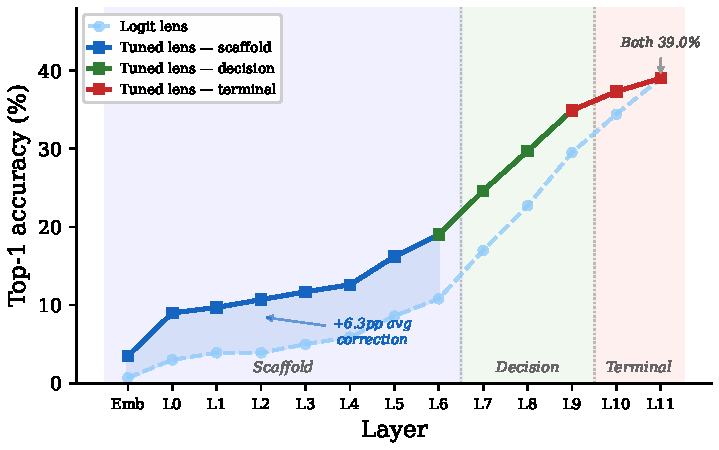
\includegraphics[width=0.85\linewidth]{fig_logit_lens.pdf}
\caption{Top-1 accuracy across layers (204,800 tokens).
The developmental arc---scaffold, decision, terminal---holds under both logit
lens (dashed) and tuned lens (solid).
The tuned lens corrects early-layer underestimates (mean $+$6.3pp at L0--L3)
while converging with the logit lens at late layers ($+$0.0pp at L11).}
\label{fig:logit_lens}
\end{figure}

The three-phase arc identified in the cross-layer MLP analysis
(\S\ref{sec:terminal}) is confirmed at the prediction level
(Figure~\ref{fig:logit_lens}):
scaffold layers gain $\sim$1--2\% top-1 accuracy per layer,
decision layers (L7--L9) gain $\sim$5--6\% per layer, and the terminal
layers (L10--L11) contribute the final push.
Only 3.0\% of tokens first reach top-1 at L11 under the tuned lens---the vast
majority of correct predictions are already in place before the final MLP acts.

\paragraph{Robustness to lens choice.}
\citet{belrose2023eliciting} showed that the logit lens underestimates early-layer
information because the residual stream has not yet rotated into the unembedding
basis.
We validate all developmental arc claims using their tuned lens---a learned affine
probe per layer, trained on held-out data to project intermediate representations
into vocabulary space without introducing extra information
(Table~\ref{tab:logit_lens}).
The tuned lens reveals substantially more information at early layers
(mean $+$6.3pp at L0--L3) while converging with the logit lens at late layers
($+$0.0pp at L11, where no rotation correction is needed).
Critically, the developmental arc is \textbf{confirmed}: decision-phase layers
gain 5.3pp/layer under the tuned lens vs.\ 1.5pp/layer in the scaffold phase
(logit lens: 6.0pp vs.\ 1.1pp).
The scaffold phase is less barren than the logit lens suggested---early layers
encode meaningful predictions that the logit lens misses---but the three-phase
structure and the decisive acceleration at L7 are robust to lens choice.

Illustrative case studies confirm three modes of factual emergence:
\textbf{(1) Easy facts arrive early:}
``Abraham $\to$ Lincoln'' locks in at L0 (99.8\% by L10; L11 MLP reduces to 99.3\%).
``William $\to$ Shakespeare'' locks in at L4 via attention copying (99.9\% by L10;
L11 MLP halves it to 54.3\%).
\textbf{(2) Medium facts require mid-layer MLPs:}
``moon'' overtakes ``planet'' at L10's MLP.
``Fahrenheit'' overtakes ``Celsius'' at L7.
\textbf{(3) Hard facts need L11 as tiebreaker:}
``second'' (speed of light), ``ic'' (DNA), and ``C'' (degrees) only reach top-1
at L11's MLP, where the exception handler makes the decisive intervention.

\subsection{L11 MLP: Helps and Hurts Simultaneously}

At scale, L11's MLP promotes 17,949 tokens to top-1 (8.8\%) while knocking
7,795 off (3.8\%), a net gain of $+$10,154 correct predictions.
But this masks a nuanced consensus-dependent effect.

At every consensus level, L11 MLP produces \emph{both} top-1 gains and losses.
Even at 7/7 consensus, it promotes 7,674 tokens while losing 3,530 (net
$+$4,144).
Yet average probability \emph{drops} at 7/7 (0.249$\to$0.178), because L11
redistributes: sharpening some predictions while smearing many others.

\begin{enumerate}
\item \textbf{At low consensus (0--3/7)}: L11 MLP is almost purely beneficial.
Average probability improves substantially at 0/7, and among tokens promoted
to top-1 at this level, fewer than 1\% are subsequently lost.

\item \textbf{At high consensus (5--7/7)}: L11 MLP makes a trade-off.
It promotes new tokens to top-1 (net positive) but degrades average probability
(net negative, $\Delta P = -0.020$ at 7/7).
At 7/7: gains 7,674 but loses 3,530.
\end{enumerate}

In Milton's \emph{Paradise Lost}, the fallen angel Moloch---``the strongest
and the fiercest Spirit''---advocates war against Heaven even when the cause is
hopeless, choosing action over abstention not from strategy but from
incapacity for restraint.
The MLP at consensus is Moloch: the routing system correctly identifies that
intervention is counterproductive on 89\% of tokens (those at 5/7 consensus
and above), but the architecture provides no bypass---every token passes
through the GELU nonlinearity, every distribution gets reshaped.
Moloch's compulsion is structural, not a bug: the MLP is architecturally
incapable of abstention.

\subsection{Consensus Predicts Helpfulness}

We verify this at scale: for 204,800 tokens, we measure whether L11's MLP
improves or degrades the probability assigned to the correct next token,
grouped by consensus level (Table~\ref{tab:consensus_help}).

\begin{table}[t]
\centering
\caption{L11 MLP effect on next-token probability by consensus level
(204,800 tokens, sequence-level bootstrap; see \S3.2).
All CIs exclude zero; crossover at 4--5/7.}
\label{tab:consensus_help}
\begin{tabular}{@{}crrrl@{}}
\toprule
Level & Tokens & Mean $\Delta P$ & 95\% CI & \\
\midrule
0/7 & 206    & $+$0.187 & [$+$0.145, $+$0.231] & \textcolor{blue}{$\blacktriangle$} \\
1/7 & 913    & $+$0.094 & [$+$0.079, $+$0.109] & \textcolor{blue}{$\blacktriangle$} \\
2/7 & 3{,}051  & $+$0.045 & [$+$0.039, $+$0.051] & \textcolor{blue}{$\blacktriangle$} \\
3/7 & 6{,}283  & $+$0.030 & [$+$0.026, $+$0.033] & \textcolor{blue}{$\blacktriangle$} \\
4/7 & 12{,}617 & $+$0.014 & [$+$0.011, $+$0.016] & \textcolor{blue}{$\blacktriangle$} \\
\midrule
5/7 & 34{,}155 & $-$0.004 & [$-$0.006, $-$0.003] & \textcolor{red}{$\blacktriangledown$} \\
6/7 & 69{,}625 & $-$0.014 & [$-$0.015, $-$0.014] & \textcolor{red}{$\blacktriangledown$} \\
7/7 & 77{,}950 & $-$0.020 & [$-$0.021, $-$0.019] & \textcolor{red}{$\blacktriangledown$} \\
\bottomrule
\end{tabular}
\end{table}

\begin{figure}[t]
\centering
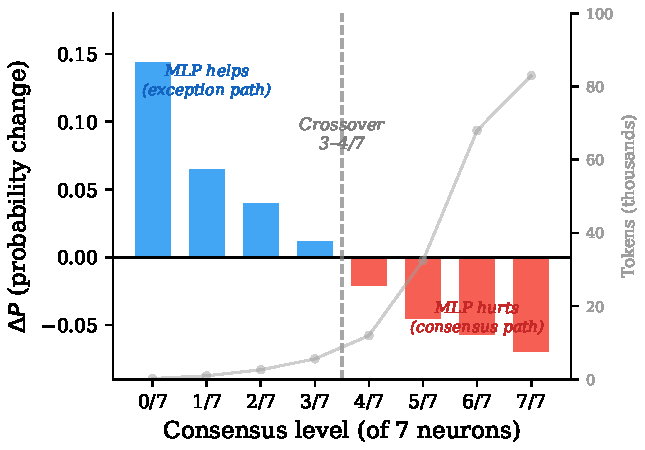
\includegraphics[width=0.85\linewidth]{fig_consensus_crossover.pdf}
\caption{L11 MLP effect on correct-token probability by consensus level
(204,800 tokens). Blue bars: MLP helps (exception path). Red bars: MLP
hurts (consensus path). The crossover between 4/7 and 5/7 closely matches the causal analysis
of \citet{balogh2026discrete}. Gray line: token count (right axis).}
\label{fig:crossover}
\end{figure}

The crossover occurs between 4/7 and 5/7 consensus
(Figure~\ref{fig:crossover}), closely matching the causal analysis of
\citet{balogh2026discrete}.
All eight bootstrap 95\% CIs (10{,}000 resamples) exclude zero:
at 4/7, the MLP still helps ($\Delta P = +0.014$, CI $[+0.011, +0.016]$),
while at 5/7 it harms ($\Delta P = -0.004$, CI $[-0.006, -0.003]$).
The crossover is statistically sharp, not gradual.
The consensus/exception routing is not merely a structural curiosity---it
is a \textbf{functional necessity} that correctly identifies when intervention
helps versus harms.

\subsection{Tier-by-Tier Ablation}

Zeroing each tier of the exception handler reveals an unexpected hierarchy
(Table~\ref{tab:ablation}, Figure~\ref{fig:tiers}).
The Core---whose ``vocabulary reset'' toward function words seemed
architecturally central---costs only $+$0.2\% PPL when removed.
The Differentiators (suppression and subword repair) are 6$\times$ more
important ($+$1.3\%).
Specialists slightly \emph{improve} PPL when ablated ($-$0.3\%), suggesting
they are marginally counterproductive on average---likely because they
fire at structural boundaries where the correct next token is highly
unpredictable, and their vocabulary push toward boundary-appropriate tokens
(paragraph markers, section headers) conflicts with the actual next token
more often than it helps.

\begin{figure}[t]
\centering
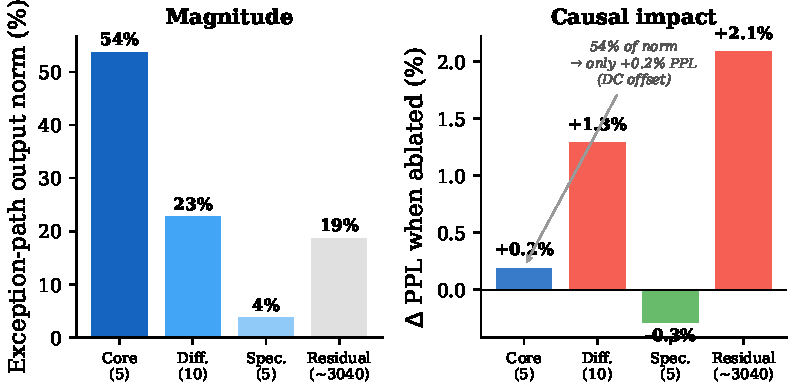
\includegraphics[width=0.95\linewidth]{fig_tier_contribution.pdf}
\caption{The DC offset paradox. \textbf{Left:} Exception-path output norm
by tier. The Core dominates at 54\%. \textbf{Right:} PPL impact when each
tier is ablated. Despite its large magnitude, the Core contributes only
+0.2\% PPL---a DC offset toward function words that the residual stream
already provides.}
\label{fig:tiers}
\end{figure}

\begin{table}[t]
\centering
\caption{PPL impact of zeroing exception handler tiers at L11's MLP
pre-activation (204,800 tokens, sequence-level bootstrap 95\% CIs from
500 sequences).}
\label{tab:ablation}
\begin{tabular}{@{}lcccc@{}}
\toprule
Tier & Neurons & PPL & $\Delta$ & 95\% CI \\
\midrule
Baseline        & ---  & 31.79 & --- & --- \\
Core            & 5    & 31.86 & $+$0.2\% & [$+$0.1\%, $+$0.4\%] \\
Differentiators & 10   & 32.20 & $+$1.3\% & [$+$0.9\%, $+$1.7\%] \\
Specialists     & 5    & 31.69 & $-$0.3\% & [$-$0.6\%, $-$0.1\%] \\
All exception   & 20   & 32.44 & $+$2.1\% & [$+$1.6\%, $+$2.5\%] \\
\bottomrule
\end{tabular}
\end{table}

Core ablation disproportionately affects low-consensus tokens ($+$2.4\% at
3/7, $-$0.4\% at 7/7), confirming that the vocabulary reset is targeted at
exception positions.
This resolves the DC offset paradox: the Core's 54\% of output norm is not
redundant---it is \emph{context-dependent}.
At low consensus (where the model is uncertain), the Core's vocabulary reset
provides a critical stable prior that the Differentiators and residual can
build upon, contributing $+$2.4\% PPL.
At high consensus (where the residual stream already has the right answer),
the same reset is counterproductive ($-$0.4\%), but the damage is small because
the residual's strong signal overwrites it.
The $+$0.2\% average impact is a Simpson's paradox: a mixture of large
positive effects on the 11\% of tokens where it matters and small negative
effects on the 89\% where it doesn't.
Gradient descent preserved this architecture not because the Core is globally
useful, but because it is \emph{locally essential} at exception positions.

The Differentiators' suppression pairs do the real work of shaping
the prediction.

\subsection{The Routing Is the Contribution}

The MLP does not retrieve knowledge---facts arrive through attention.
At every ``aha'' layer where a correct prediction first locks in, we find
a specific attention head copying from the semantically relevant source token.
L11's H8 stands out: with near-zero BOS attention, it attends to content
words (\texttt{freezes}, \texttt{Einstein}, \texttt{Revolution}) while all
other L11 heads are BOS sinks ($>$0.80 to position 0).
This single head provides the factual signal that the MLP then amplifies or
suppresses based on its routing decision.

The routing is legible: 27 named neurons with documented behavior,
summarized as pseudocode in Figure~\ref{fig:pseudocode}.
The knowledge it routes around is not.

Having characterized L11's architecture---its tiers, its consensus detector,
its relationship to knowledge---we now ask: is this structure unique to the
terminal layer, or does it appear throughout the model?

%=============================================================================
\section{Terminal Crystallization}
\label{sec:terminal}
%=============================================================================

\subsection{Earlier Layers Lack Structure}

We replicated the full characterization at L7 (1 consensus neuron) and L10
(3 consensus neurons).
Neither shows the structured exception handler found at L11
(Table~\ref{tab:cross_layer}).

\begin{table}[t]
\centering
\caption{Exception handler structure across all 12 layers (102,400 tokens).
Max Jaccard is the highest pairwise co-firing similarity with the most
anticorrelated neuron. Only L11's known architecture (rightmost column)
shows tight co-firing (0.998), selective fire rate (11.3\%), and strong
enrichment (2.0$\times$). No other layer approaches this structure.}
\label{tab:cross_layer}
\small
\begin{tabular}{@{}lcccccc@{}}
\toprule
 & L0--L3 & L4--L6 & L7--L9 & L10 & L11 (auto) & L11 (known) \\
\midrule
Exc.\ fire rate & 6--15\% & 12--15\% & 25--36\% & 38.5\% & 10.9\% & 11.3\% \\
Max Jaccard     & 0.06--0.16 & 0.13--0.18 & 0.26--0.36 & 0.384 & 0.123 & \textbf{0.998} \\
Enrichment      & 1.06--1.17$\times$ & 1.11--1.21$\times$ & 1.06--1.09$\times$ & 1.05$\times$ & 1.15$\times$ & \textbf{2.0$\times$} \\
Hi-Jaccard ($>$0.5) & 0 & 0 & 0 & 0 & 0 & \textbf{4} \\
\bottomrule
\end{tabular}
\end{table}

A survey across all 12 layers (Table~\ref{tab:cross_layer}) confirms that
L11's structure is unique.
The highest Jaccard similarity found by automated search at \emph{any} layer
is 0.384 (L10).
L11's known Core achieves 0.998---a qualitative gap, not a quantitative one.
No other layer shows Specialist neurons, suppression pairs, or enrichment
above 1.21$\times$.

\subsection{Why the Terminal Layer?}

We hypothesize that legible routing crystallizes at L11 because it is the
\textbf{last opportunity} for the model to adjust its prediction.
Earlier layers can afford diffuse, distributed processing because subsequent
layers can correct errors.
L11 has no safety net---its decisions are final.
This produces gradient pressure for clear, reliable routing at the terminal
layer.

\textbf{Testable prediction:} In deeper models (e.g., GPT-2 Medium at 24
layers, GPT-2 Large at 36), equivalent consensus-exception structure should
appear at the final MLP layer, not at L11.
If terminal crystallization is driven by ``last opportunity'' pressure, the
structure should track model depth, not absolute layer index.

\subsection{L11H7: The Dominant Attention Head}

The most important attention head at L11 is H7, measured by mean absolute
attention-weighted value norm across 204,800 tokens
(score 91.5, 6$\times$ the next head).
H7 sends 45.4\% of its weight to the BOS token.
Exception tokens attend to BOS even more (47.0\% vs 37.3\% for high-consensus
tokens) and with lower entropy (3.01 vs 3.51 bits).

This is the attention sink phenomenon \citep{xiao2023efficient}:
when the MLP handles the real work (exception path), the attention head has
nothing to contribute and dumps weight on the no-op BOS position.

%=============================================================================
\section{Discussion}
%=============================================================================

\subsection{The Program and the Database}

Our decomposition separates GPT-2's L11 MLP into two functionally distinct
components:

\begin{enumerate}
\item \textbf{The Program} (27 named neurons): Binary routing logic that
determines processing path, resets vocabulary, suppresses candidates, and detects
boundaries. Fully legible as pseudocode.

\item \textbf{The Database} ($\sim$3{,}040 residual neurons): Contextual adjustment
signals that interact with knowledge already in the residual stream. Distributed
and not directly legible, but the \emph{mechanism} is legible.
\end{enumerate}

The analogy is a software system where the control flow is open-source
but the database is encrypted:
the routing logic is legible even when the data it operates on is not.

\subsection{What the Exception Handler Does Not Detect}
\label{sec:garden_path}

The exception handler detects subword fragments, structural breaks, and rare
tokens (\S\ref{sec:exception}).
A natural hypothesis---motivated by psycholinguistic accounts of garden-path
processing \citep{frazier1982making}---is that it also detects
\emph{syntactic reparse}: moments when the model must revise a
structural commitment, as in garden-path sentences.

\paragraph{Experiment.}
Following \citet{vangompel2001lexical}, we constructed 15 minimal pairs
contrasting intransitive verbs (which create garden paths in human reading)
with transitive verbs (which do not):

\begin{quote}
\emph{After the dog \textbf{struggled} the vet took off the muzzle.} \\
\emph{After the dog \textbf{scratched} the vet took off the muzzle.}
\end{quote}

\noindent In the intransitive version, ``the vet'' is temporarily ambiguous---human
readers initially parse it as the object of ``struggled'' (late closure), then
must reparse at ``took'' when the main clause begins.
At this disambiguation point, we measured surprisal, L11 consensus level, N2123
activation, and MLP delta norm.

\paragraph{Results: reversed garden-path effect.}
We found no evidence of differential N2123 response (mean activation 0.102 intransitive vs.\ 0.105 transitive,
$t(14) = -0.45$, $p = 0.66$).
With $N = 15$ pairs, a post-hoc power analysis (two-sided $t$-test, $\alpha = 0.05$, $\sigma = 0.1$) yields 80\% power to detect effects of $d \geq 0.78$ --- we are powered only for large effects and cannot rule out small-to-medium N2123 sensitivity to syntactic reparse.
Consensus, surprisal, and MLP delta are also nonsignificant (all $p > 0.27$).
Only 1 of 4 directional predictions was confirmed.

The \emph{reversed} surprisal pattern is more interesting: the transitive
condition produces \emph{higher} surprisal at disambiguation.
For ``struggled/scratched,'' surprisal at ``took'' is 5.4 bits
(intransitive) vs.\ 11.6 bits (transitive).
This reversal is consistent across multiple items (``sneezed'' 6.8 vs.\
``visited'' 16.2 bits; ``slept'' 13.2 vs.\ ``ignored'' 11.3 bits).
A paired Wilcoxon signed-rank test across all 15 pairs shows the transitive
condition produces significantly higher surprisal at disambiguation
($W = 12$, $p = 0.018$, median difference $+$3.1 bits).
The reversed garden-path effect is statistically reliable, even though N2123
does not detect it.

\paragraph{Interpretation: one-stage parsing.}
GPT-2 does not garden-path in the way humans do.
When it encounters an intransitive verb like ``struggled,'' it uses
subcategorization information \emph{immediately}---knowing ``struggled'' cannot
take a direct object, it parses ``the vet'' as the subject of a new clause
from the start.
When it encounters a transitive verb like ``scratched,'' it commits to the
object reading for ``the vet,'' and must revise at ``took''---producing the
high surprisal.
The garden-path effect exists in GPT-2 but is \textbf{reversed}: it is the
transitive, not intransitive, condition that creates the garden path.

This is consistent with the exception handler operating at the level of
\emph{token-level predictability}, not \emph{syntactic structure}.
N2123 fires when the model doesn't know what kind of token comes next---an
uncertainty about \emph{vocabulary}, not about \emph{parse}.
Syntactic reparse, when it occurs, is handled incrementally by attention
and does not register as an exception at L11's MLP.

\paragraph{Connection to selective context override in humans.}
\citet{britt1992parsing} showed that even human garden-path effects are
selectively modular: discourse context can override PP attachment preferences
(shallow, within-phrase ambiguity) but \emph{cannot} override reduced relative
clause preferences (deep, cross-clause ambiguity requiring a new S node).
Our verb subcategorization ambiguity is structurally analogous to the
reduced relative case---it involves clause-level reparse (``the vet'' as
subject of a new clause vs.\ object of the current one).
That GPT-2 resolves this ambiguity immediately via subcategorization,
without N2123 involvement, suggests an architecture where deep structural
decisions operate autonomously from the exception handler---paralleling
Britt et al.'s Cooperative Language Processor, where clause-level parsing
resists contextual override precisely because it is handled by an
autonomous syntactic component.

\subsection{Implications for Efficiency}

Silencing Moloch---bypassing the MLP entirely for the 89\% of tokens at
5/7 consensus and above---would save the vast majority of MLP compute at
L11 while \emph{improving} prediction quality on those tokens.
Even the conservative target of 7/7 consensus (40\% of tokens) costs only
6.9\% PPL when bypassed, while zeroing MLP contributions for consensus tokens
across layers L7--L11 cumulatively costs 11.8\%.
Linear approximation (skipping GELU) is catastrophically wrong, confirming that
the MLP implements a binary switch rather than a smooth nonlinearity.

\subsection{Controls}
\label{sec:controls}

\paragraph{Null model.}
Could the tier architecture be an artifact of fire-rate binning---i.e., would
\emph{any} MLP show apparent structure if we group neurons by activation
magnitude?
We ran identical analysis on a randomly initialized GPT-2 (same architecture,
untrained weights).
The random model shows no consensus-exception structure:
the exception neuron fires on $\sim$64\% of tokens (vs.\ 11.3\% trained),
Core Jaccard similarity is 0.53 (vs.\ 0.86 trained, min 0.68),
and exception rate is \emph{flat} across consensus levels
(63--65\%, no anticorrelation; trained: 98\% at 0/7 $\to$ 65\% at 7/7).
The three-tier architecture is entirely absent in untrained weights.

\paragraph{Threshold robustness.}
\label{sec:threshold}
We swept the binary firing threshold across two orders of magnitude
($\theta \in \{0.01, 0.05, 0.1, 0.25, 0.5, 1.0\}$).
Core co-firing (Jaccard $\geq 0.45$) and consensus-exception anticorrelation
(spread $\geq 0.11$) persist across all thresholds.
The strongest anticorrelation appears at $\theta = 0.25$ (spread 0.81),
with the canonical $\theta = 0.1$ lying in a stable plateau.
No threshold produces qualitatively different structure---the findings are not
an artifact of the 0.1 cutoff.

\begin{table}[t]
\centering
\caption{Enrichment of routing neurons under exception firing
(one-sided Fisher's exact test, Bonferroni-corrected $\alpha = 1.6 \times 10^{-5}$).
N2123 has a generic activation rate of 70.9\% ($|\text{GELU}| > 0.1$), but only 11.3\% of tokens produce the high-magnitude activations that indicate exception-path routing (\S\ref{sec:exception}). The enrichment analysis here uses the generic threshold; the 1.41$\times$ enrichment reflects the concentration of high-activation events within exception tokens.}
\label{tab:enrichment_stats}
\begin{tabular}{@{}llrrrr@{}}
\toprule
Neuron & Tier & Base rate & Exc rate & Enrichment & $p$-value \\
\midrule
N2123 & Core           & 70.9\% & 100.0\% & 1.41$\times$ & $< 10^{-300}$ \checkmark \\
N584  & Differentiator & 6.2\%  & 8.3\%   & 1.33$\times$ & $< 10^{-300}$ \checkmark \\
N2378 & Differentiator & 5.7\%  & 7.4\%   & 1.30$\times$ & $< 10^{-300}$ \checkmark \\
N737  & Specialist     & 4.0\%  & 4.9\%   & 1.22$\times$ & $< 10^{-300}$ \checkmark \\
N1602 & Differentiator & 22.7\% & 24.4\%  & 1.08$\times$ & $< 10^{-300}$ \checkmark \\
N611  & Differentiator & 67.2\% & 71.8\%  & 1.07$\times$ & $< 10^{-300}$ \checkmark \\
\midrule
\multicolumn{2}{@{}l}{Consensus neurons (5 of 7)} & \multicolumn{2}{c}{---} & 0.96--1.01$\times$ & $> 0.05$ \\
\multicolumn{2}{@{}l}{Remaining routing (15)} & \multicolumn{2}{c}{---} & 0.98--1.01$\times$ & $> 0.01$ \\
\bottomrule
\end{tabular}
\end{table}

\subsection{Limitations}

\begin{itemize}
\item \textbf{Single model}: All analysis is on GPT-2 Small (124M parameters).
The terminal crystallization hypothesis predicts that the same structure
appears at the final layer of deeper models, but this is untested.
\item \textbf{Single domain}: All experiments use WikiText-103 (encyclopedic
prose). The consensus neuron characterizations (``clausal continuation,''
``sequential structure'') may not hold for dialogue, code, poetry, or
legal text. A cross-domain validation would strengthen or scope the claims.
\item \textbf{Single layer depth}: We characterize L11 comprehensively but only
sketch L7 and L10.
\item \textbf{Garden-path stimuli}: Our 15 sentence pairs
(\S\ref{sec:garden_path}) test a limited range of syntactic constructions;
more complex garden paths (e.g., reduced relatives) may produce different
patterns.
\item \textbf{BPE confounds}: In some garden-path pairs, the
disambiguation word falls at different absolute positions due to BPE
tokenization, potentially confounding position-sensitive effects.
\item \textbf{Activation transplant}: The $N = 5$ transplant experiment
(\S\ref{sec:knowledge_neurons}) is underpowered; we treat it as a
consistency check, not standalone evidence.
\end{itemize}

%=============================================================================
\section{Conclusion}
%=============================================================================

The final MLP of GPT-2 Small implements a legible routing program:
7 consensus neurons detect ``normal language'' along distinct linguistic
dimensions, a single exception neuron reliably indicates which of
two processing paths is active---a three-tier exception handler or quiet
pass-through---and $\sim$3{,}040 residual neurons provide contextual adjustments
to knowledge already present in the residual stream.
This architecture crystallizes only at the terminal layer.

The MLP's contribution is not knowledge retrieval but \textbf{routing}:
deciding whether to intervene or abstain.
The exception handler's scope is sharply bounded:
it detects token-level vocabulary uncertainty---subword fragments,
structural breaks, rare patterns---but not syntactic reparse.
The garden-path experiment makes this concrete: GPT-2 uses verb
subcategorization immediately (``struggled'' $\neq$ ``scratched'' from the
first token of the ambiguous NP), producing a \emph{reversed} garden-path
effect where the transitive, not intransitive, condition generates the garden
path.
Whether this extends to other syntactic constructions and larger models remains
to be tested.
For the verb subcategorization ambiguities we tested ($N = 15$ pairs),
GPT-2 Small behaves as a one-stage parser---it does not build tentative
structures and revise them, but commits incrementally using all available
lexical information.
Whether this extends to other syntactic constructions (reduced relatives,
NP/S ambiguities, attachment ambiguities) and larger models is an open
question that our stimuli cannot answer.
For the constructions tested, the exception handler fires on vocabulary
uncertainty, not parse ambiguity, because the model never enters the ambiguous
parse state that would require an exception.

\paragraph{Implications.}
For \textbf{efficiency}: bypassing the MLP for high-consensus tokens
(40\% of traffic at 7/7) costs only 6.9\% PPL while saving the full
MLP forward pass---a principled, routing-aware alternative to speculative
decoding.
For \textbf{model editing}: the finding that ``knowledge neurons'' are routing
infrastructure reframes ROME and related methods---weight edits succeed by
changing routing decisions, not by modifying stored facts.
This predicts that edits should generalize across phrasings (the routing
is content-independent) but fail across domains where the routing structure
differs.
For \textbf{scaling}: if terminal crystallization is driven by last-opportunity
gradient pressure, it should track model depth rather than absolute layer index.
GPT-2 Medium (24 layers) and Large (36 layers) provide immediate test cases.

We can read 27 neurons as a routing program.
The 3{,}040 neurons they route remain opaque.

\bibliography{references}
\bibliographystyle{plainnat}

\end{document}
